\documentclass[crop,tikz]{standalone}% 'crop' is the default for v1.0, before it was 'preview'
%\usetikzlibrary{...}% tikz package already loaded by 'tikz' option
\usetikzlibrary{shapes,snakes}
\usepackage{amsmath}
\begin{document}
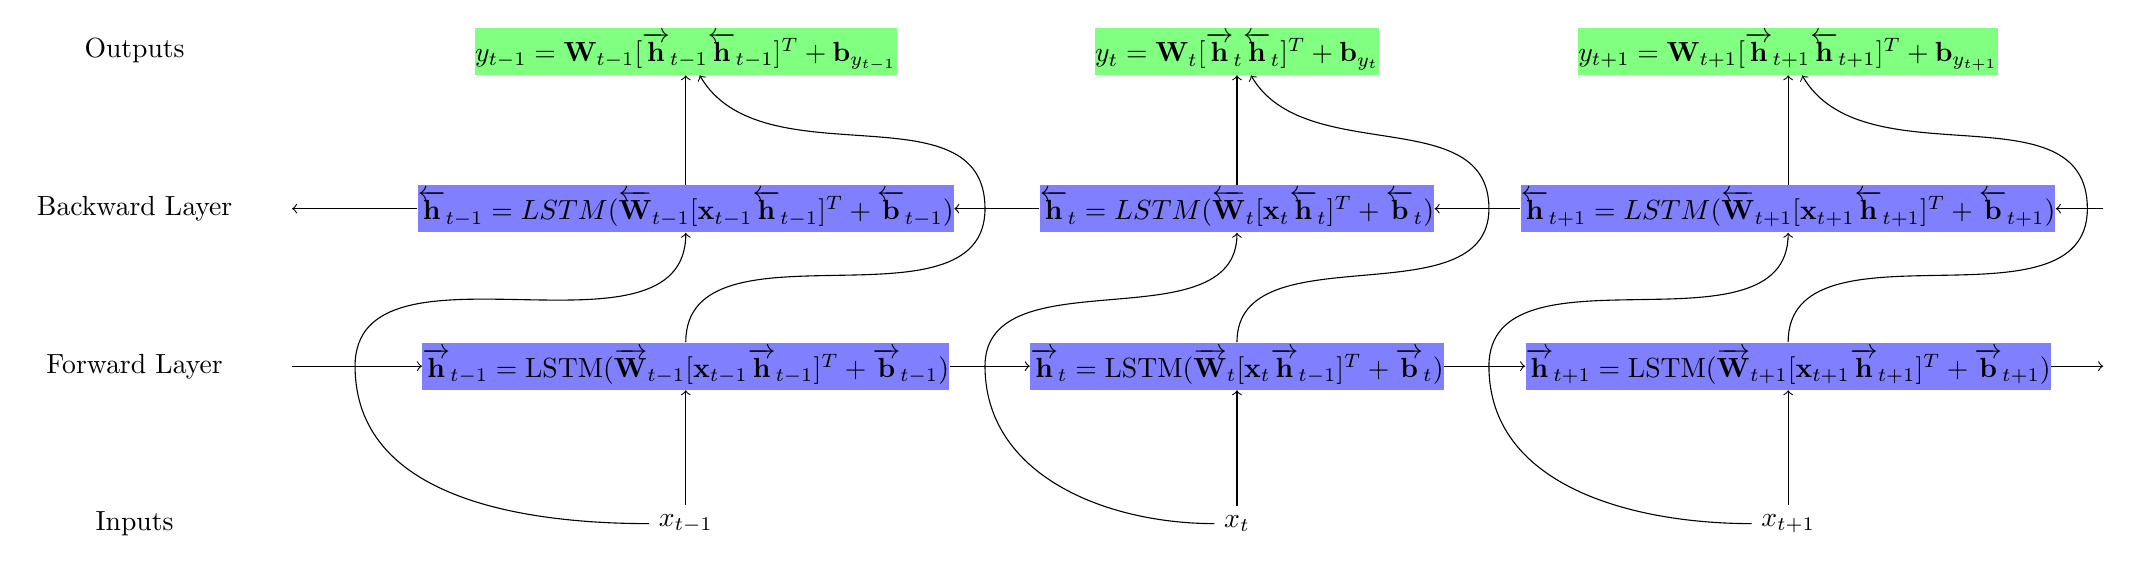
\begin{tikzpicture}

\def\layersep{7.0cm}

\tikzstyle{rcNeuron}=[rectangle,fill=black!25,minimum size=17pt,inner sep=0pt]
\tikzstyle{LSTM}=[rcNeuron, fill=blue!50];
\tikzstyle{neuron}=[rectangle,fill=black!25,minimum size=17pt,inner sep=0pt]
\tikzstyle{linearNeuron}=[neuron, fill=green!50];
%Layer Marks
\node (outputLabel)   at (0,6) {Outputs};
\node (backwardLabel) at (0,4) {Backward Layer};
\node (forwardLabel)  at (0,2) {Forward Layer};
\node (inputLabel)    at (0,0) {Inputs};

%input nodes.
\node (xtm1) at (\layersep,0) {$x_{t-1}$};
\node (xt)   at (2*\layersep,0) {$x_{t}$};
\node (xtp1) at (3*\layersep,0) {$x_{t+1}$};

%output nodes
\node[linearNeuron] (ytm1) at (\layersep,6) {$y_{t-1}  = \mathbf{W}_{t-1} [ \overrightarrow{\mathbf{h}}_{t-1} \overleftarrow{\mathbf{h}}_{t-1}]^T+ \mathbf{b}_{y_{t-1}}$};
\node[linearNeuron] (yt)   at (2*\layersep,6) {$y_{t} = \mathbf{W}_{t} [ \overrightarrow{\mathbf{h}}_{t} \overleftarrow{\mathbf{h}}_{t}]^T + \mathbf{b}_{y_{t}}$};
\node[linearNeuron] (ytp1) at (3*\layersep,6) {$y_{t+1} =  \mathbf{W}_{t+1} [ \overrightarrow{\mathbf{h}}_{t+1} \overleftarrow{\mathbf{h}}_{t+1}]^T+ \mathbf{b}_{y_{t+1}} $};

% forward lstm blocks.
\node[LSTM] (forwardXtm1) at (\layersep,2) {$\overrightarrow{\mathbf{h}}_{t-1} = \text{LSTM}(\overrightarrow{\mathbf{W}}_{t-1} [\mathbf{x}_{t-1} \overrightarrow{\mathbf{h}}_{t-1}]^T + \overrightarrow{\mathbf{b}}_{t-1})$};
\node[LSTM] (forwardXt) at (2*\layersep,2) {$\overrightarrow{\mathbf{h}}_{t} = \text{LSTM}(\overrightarrow{\mathbf{W}}_{t} [\mathbf{x}_{t} \overrightarrow{\mathbf{h}}_{t-1}]^T + \overrightarrow{\mathbf{b}}_{t})$};
\node[LSTM] (forwardXtp1) at (3*\layersep,2) {$\overrightarrow{\mathbf{h}}_{t+1} = \text{LSTM}(\overrightarrow{\mathbf{W}}_{t+1} [\mathbf{x}_{t+1} \overrightarrow{\mathbf{h}}_{t+1}]^T + \overrightarrow{\mathbf{b}}_{t+1})$};

% backward lstm blocks.
\node[LSTM] (backwardXtm1) at (\layersep,4) {$\overleftarrow{\mathbf{h}}_{t-1} = LSTM(\overleftarrow{\mathbf{W}}_{t-1} [\mathbf{x}_{t-1} \overleftarrow{\mathbf{h}}_{t-1}]^T + \overleftarrow{\mathbf{b}}_{t-1})$};
\node[LSTM] (backwardXt) at (2*\layersep,4) {$\overleftarrow{\mathbf{h}}_{t} = LSTM(\overleftarrow{\mathbf{W}}_{t} [\mathbf{x}_{t} \overleftarrow{\mathbf{h}}_{t}]^T + \overleftarrow{\mathbf{b}}_{t})$};
\node[LSTM] (backwardXtp1) at (3*\layersep,4) {$\overleftarrow{\mathbf{h}}_{t+1} = LSTM(\overleftarrow{\mathbf{W}}_{t+1} [\mathbf{x}_{t+1} \overleftarrow{\mathbf{h}}_{t+1}]^T + \overleftarrow{\mathbf{b}}_{t+1})$};

% connections
\draw[->] (2,2)         -- (forwardXtm1);
\draw[->] (forwardXtm1) -- (forwardXt);
\draw[->] (forwardXt)   -- (forwardXtp1);
\draw[->] (forwardXtp1) -- (25,2);

\draw[->] (backwardXtm1) -- (2,4);
\draw[->] (backwardXt) -- (backwardXtm1);
\draw[->] (backwardXtp1) -- (backwardXt);
\draw[->] (25,4) -- (backwardXtp1);

\draw[->] (xtm1) -- (forwardXtm1);
\draw[->] (xt) -- (forwardXt);
\draw[->] (xtp1) -- (forwardXtp1);

\draw[->] (xtm1) to[out=180,in=-90] (2.8,2) to[out=90,in=270] (backwardXtm1);
\draw[->] (xt) to[out=180,in=-90] (10.8,2) to[out=90,in=270] (backwardXt);
\draw[->] (xtp1) to[out=180,in=-90] (17.2,2) to[out=90,in=270] (backwardXtp1);

\draw[->] (forwardXtm1) to[out=90,in=270] (10.8,4) to[out=90,in=300] (ytm1);
\draw[->] (forwardXt) to[out=90,in=270] (17.2,4) to[out=90,in=300] (yt);
\draw[->] (forwardXtp1) to[out=90,in=270] (24.8,4) to[out=90,in=300] (ytp1);

\draw[->] (backwardXtm1) -- (ytm1);
\draw[->] (backwardXt) -- (yt);
\draw[->] (backwardXtp1) -- (ytp1);

\end{tikzpicture}
\end{document}